%%% bandwidth-mining.tex: -*- LaTeX -*-  DESCRIPTIVE TEXT.
%%% 
%%% Copyright (c) 2017 Brian J. Fox & Orchid Labs, Inc.
%%% Author: Brian J. Fox (bfox@meshlabs.org)
%%% Author: A truckload of others
%%% Birthdate: Tue Oct 10 12:03:25 2017.

\begin{figure}[htbp]
  \centering
  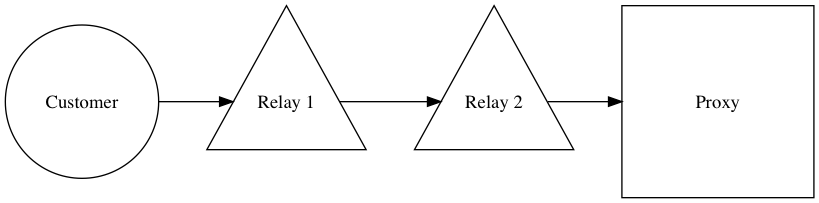
\includegraphics[width = 300pt]{sttc}
  \caption{A three-Econ Manifold routing traffic for a Customer}
\end{figure}

In this section we will describe the specification for Relay and Proxy
behavior, and discuss the ``chaining together'' of these nodes to
support uncensorable, anonymous web browsing.

\subsection{Specification for the Sale of Bandwidth}

Relay nodes implement a relatively simple behavior pattern:

\begin{itemize}
\item Maintain one or more connections, each with their own encryption key.
\item Check any tickets received, and cash-in winners.
\item Monitor the balance of trade, and disconnect if it exceeds a
  predeclared amount.
\item Receive data from any open connection, and perform decryption at
  message boundaries.
\item Process decrypted messages as follows:
  \begin{itemize}
  \item Forward any non-control segments to the connection(s)
    specified in the message.
  \item Process any control segments:
    \begin{itemize}
    \item \emph{Dummy Data.} Instructs the Relay to discard this segment.
    \item \emph{Burn at Rate.} Instructs the Relay to send data over a
      connection at a fixed rate, queueing packets and generating data
      as necessary to maintain the rate.
    \item \emph{Ratchet Ticket.} Instructs the Relay to pass a Ticket to
      the peer it received this packet from.
    \item \emph{Initiate Connection.} Instructs the Relay to establish a
      new connection. Used during setup and to handle disconnection.
    \item \emph{Initial Web Connection.} (Proxies Only.) Instructs the
      proxy to open an SSL connection to the specified host. To
      support whitelists, this cannot be a raw IP address.
    \end{itemize}
  \end{itemize}
\end{itemize}

%% [saurik: should we flesh out the above with packet specifics? I feel
%%   like *this* part of the document can/should be more specific than
%%   the rest, as we'd like transient nodes to be written more rapidly
%%   than full clients? Just a guess. - dls]

An important consideration in the above behavior is that no
proof-of-work is required of Relays on an ongoing basis. When combined
with all our connections being WebRTC connections, this leaves the
door open for websites potentially monetizing their visitors by
running pure javascript relay code.

For discussion of possible extensions via application specific control
segments, see Section \ref{sec:future}.

\subsection{Guard Nodes and ``Bandwidth Burning''}
\label{bandwidth-burning}

The relay that a customer is connected to has a very important piece
of information: the customer’s IP address. We assume customers will
want to keep this as private as possible, and so the default client
expresses a preference for long-lived peers as the first
hop.

Another concern for nodes at the first hop, which is discussed in
depth in our discussion of informational attacks stemming from
collusion (Section \ref{sec:collusion}), is they sit in an ideal
position to perform timing attacks. To prevent these attacks, we
recommend that privacy-conscious users employ a method called
\emph{Bandwidth Burning} -- paying the second hop to send a fixed
amount of bandwidth to the customer. As this approach results in
data-usage which is completely uncorrelated to network usage, this
approach prevents timing attacks performed by adversaries which cannot
see the inbound traffic of relay three.

To provide assistance to users seeking evasion (Section
\ref{sec:evasion}), bandwidth burning will also support non-fixed
rates determined by the statistical properties of popular non-\Orchid
WebRTC protocols.

\subsection{Chaining}

Customers interested in employing Relays for anonymous Internet
access, will use the above specification to create ``chains'' of
relays.

